\chapter{Models of Steganography}
\label{chap:models}
After the previous chapter introduced all necessary notions concerning
cryptography, this chapter deals with the formal definitions of
\emph{provably secure steganography}. Throughout this thesis, we will
use multiple different models of steganography, that mainly differ in
three aspects:
\begin{description}
\item[Efficiency:] The first formal definition of provably secure
  steganography was given by \citeauthor{hopper2009provably} in
  \cite{hopper2009provably}, the running time of a stegosystem was
  not necessarily efficient, \ie not bounded by a polynomial in the
  security parameter $\kappa$. While some subsequent works defined
  efficiency as a requirement (see \eg \cite{backes2005active,
    dedic2009lower}), \citeauthor{hopper2009provably} make use of the
  fact that their stegosystems may run for a long time to obtain their
  results. We thus distinguish between the original definition -- which
  we will call \myDefInformal{non-efficient stegosystems} -- and the
  updated notion \myDefInformal{efficient stegosystems}. 
\item[Applicability:] A typical problem that arises when one designs a stegosystem
  concerns their \emph{applicability}: On which kind of channels should
  or stegosystem work? One could for example design a stegosystem that
  works for a concrete channel where the documents are $200$ \acs{JPEG}
  pictures of size $600\times 600$ pixels that we know in
  beforehand. \myNote{This nomenclature is taken from
    \cite{liskiewicz2013grey}.}
Such a stegosystem is called a \myDefInformal{white-box
    stegosystem}, as the stegosystem has complete knowledge of the
  channel. Typically one wants to design more general stegosystems. For
  example, it might be appropriate to design a stegosystem that works
  for all channels that contain \acs{JPEG} pictures of size $600\times
  600$ pixels. As the stegosystem still has some knowledge about the
  documents, such a system is called a \myDefInformal{grey-box
    stegosystem}. The most general form of a stegosystem is a
  stegosystem that works \emph{on every channel} (containing
  sufficiently many documents). We call such a system a
  \myDefInformal{universal stegosystem} or a \myDefInformal{black-box
    stegosystem}. As we try to give as general results as possible in
  this thesis, we will develop grey-box or black-box stegosystems for
  our positive results and rule out white-box stegosystems for our
  negative results.
\item[Key-Symmetry:] As in the cryptographic setting, the stegoencoder
  needs a key $k$ to encode the message into the channel  and the
  stegodecoder also needs a key $k'$. If $k=k'$ we speak of a
  \myDefInformal{symmetric-key stegosystem} or \myDefInformal{secret-key
    stegosystem}. In contrast, if $k\neq k'$ and $k$ is publicly known
  and $k'$ is kept secret, we call such a system a
  \myDefInformal{public-key stegosystem}. Furthermore, we denote the
  publicly known key $k$ as $\pk$ (for public key) and the secret key
  $k'$ as $\sk$ (for secret key). Depending on the setting we will also
  analyze different security notions. 
\end{description}

To help the reader to keep track which of these $2\cdot 3\cdot 2=12$
configurations we currently use, the names of the chapters typically
contain all information about the notions used in the chapter. We will
also always give a short description about these aspects in the first
few sentences of the chapter.

\section{Unsuspicious Communication}
In order to formalize that the output of a secure stegosystem is
indistinguishable from unsuspicious communication, we first need a mean
to define this unsuspicious communication. We will do this via the
notion of a \emph{channel}. We will think of this unsuspicious
communication as the unidirectional transmission of \emph{documents}
from Alice to Bob and will model this as a probability distribution upon
those documents. This distribution indicates the probability that Alice
sends a certain document to Bob. There are two more things we need to
consider to make this model realistic and useful for us. First, the
probabilities may change over the time depending on the already sent
documents. If Alice sends Bob a postcard from the beach, it is quite
unlikely (though not impossible) that the next postcard that Bobs get
will come from the Antarctic. This change of the probability
distribution will be reflected by something we call the \emph{history}
-- the sequence of already transmitted documents. Second, larger
security parameters typically allow us to send larger messages. Hence,
the amount of information needed to hide those messages also grows. 
To hide those messages, there are to approaches to handle the need for
more information:
\begin{itemize}
\item In the first approach used by \citeauthor{hopper2009provably} in
  \cite{hopper2009provably}, it is assumed that the size of the
  documents is independent from the security parameter and thus treated
  as a constant. In order to have a large enough entropy to handle
  larger messages, \citeauthor{hopper2009provably} do not deal with
  single documents, but rather with sequences of documents of sufficient
  length. This model was criticized by
  \citeauthor{lysyanskaya2006imperfect} in
  \cite{lysyanskaya2006imperfect} as one should only be able to look at
  the distribution with history $h$ containing the document $d$
  \emph{after} the document $d$ was transmitted to Bob especially if the
  the size of documents is very small.
\item In the second approach that we will use, we assume that the size
  of the document depends on the security parameter, \ie the entropy of
  a single document is high enough already. This approach is more
  general then the first one as we will simply interpret a sequence of
  constant-sized objects as a single document. This simplifies the
  analysis and our notation as we can always directly talk about
  documents and not about sequences.
\end{itemize}

\begin{example}
  Let us look at the example that Alice send Bob pictures from her
  holiday. Suppose that every picture is encoded in \acs{JPEG} and of
  size $600\times 600$ pixels. Denote the set of all such pictures by
  $\Pics$. Furthermore suppose that on security
  parameter $\kappa$, we want to embed messages of length $m(\kappa)$. 

  In the first approach, a document $d$ would consist of a \emph{single}
  picture, \ie $d\in \Pics$ and we would only deal with sequences of
  pictures of length $\approx m(\kappa)$. Hence, our channel would be a
  probability distribution on $\Pics$, but our stegosystem would only
  deal with sequences taken from this distribution.

  In the second approach, a document $d$ would already consists of sequence
  of pictures, \ie $d\in \Pics^{m(\kappa)}$. Hence, our channel would be a
  probability distribution on $\Pics^{m(\kappa)}$ and our stegosystem would
  also directly deal with elements of this distribution. 
\end{example}

Formally, a \myDef{channel} $\chan$ on the alphabet $\Sigma$ is a
function that maps an element $h\in \Sigma^{*}$ -- the \myDef{history}
-- and a number $n\in \nats$ -- the \myDef{document length} -- to a
probability distribution on $\Sigma^{n}$. We will denote this
probability distribution by $\chan_{h,n}$ instead of
$\chan(h,n)$. An element of $\Sigma^{n}$ is called a \myDef{document} or
\myDef{covertext}. Typically, we will implicitly assume that
$\Sigma=\{0,1\}$ to simplify the following analysis concerning the
amount of information that is present in the channel $\chan$. The
\myDef{min-entropy of a channel} $\minent(\chan,n)$ for
a channel $\chan$ and a natural number $n\in \nats$ is defined as
$\minent(\chan,n) = \min_{h\in \Sigma^{*}}\{\minent(\chan_{h,n})\}$. As
demonstrated in \cite{hopper2009provably}, the number of bits embeddable
in a \emph{single document} is bounded by $\minent(\chan,n)$. 

Note that some works (\eg \cite{hopper2009provably,liskiewicz2013grey})
also limit the histories to those that actually may occur. They call
those histories \myDef{legal histories}. While it may seem useful to
limit the used histories in such a way, several problems arise from it
such as:
\begin{itemize}
\item What happens if the stegosystems sends an ``illegal'' document,
  that is not recognized as such by the warden?
\item How can a warden make sure that he only chooses legal histories?
\end{itemize}
Answering these questions in a completely satisfactory way seem to lead
to a change in the steganographic model. To the best of our knowledge,
the works that use the notion of legal histories also ignore these
problems. We thus decided to also ignore this issue by removing this
complicated restriction from our work. 

\section{Stegosystems}
We are now able to finally describe the notion of a stegosystem. As
discussed in the beginning of the section, we will follow the definition
of \cite{hopper2009provably} and will not assume that a stegosystem
needs to run in polynomial time. In order to reduce the redundancy of
this work, we will only define secret-key stegosystems and then
explain the (relatively minor) differences to public-key systems later
on. Let $\mu,n$ and $\ell$ be polynomials throughout this chapter that
will model that the stegoencoder upon security parameter $\kappa$ takes
a message of length $\mu(\kappa)$ and embeds it into $\ell(\kappa)$
documents of length $n(\kappa)$. We thus call $\mu$ the \myDef{message
  length}, $n$ the \myDef{document length} and $\ell$ the \myDef{output
  length} of the stegosystem. 


A \myDef{(secret-key) stegosystem}
$(\Gen,\SEnc,\SDec)$ is a triple of \acp{PTM} such that the algorithm
$\Gen(1^{\kappa})$ produces a key $k\in \{0,1\}^{\kappa}$.
The \myDef{stegoencoder} $\SEnc$ takes as input the key $k$, a
message (the \myDef{hiddentext}) $m\in \{0,1\}^{\mu(\kappa)}$, a history $h\in
\DomainHistory$ and some state information $s\in
\{0,1\}^{*}$ and outputs a \emph{single document} (the
\myDef{stegotext}) $d\in
\Sigma^{n(\kappa)}$ and updated state information $s'\in
\{0,1\}^{*}$. Its goal is to embed a piece of $m$ into the document
$d$. It will also have access to samples of the probability distribution
$\chan_{h,n(\kappa)}$. The complete output of the run of the
stegoencoder is denoted by $\SEnc^{\chan}(k,m,h)$ and defined by the
following scheme:
\myAlgorithm{$\SEnc^{\chan}(k,m,h)$}{Key $k$, message $m$, history $h$}{
\State $s := \varnothing$ \Comment{initialize the empty state}
\For{$i=1,2,\ldots,\ell(\kappa)$}
\State $(d_{i},s) \gets \SEnc^{\chan_{h,n(\kappa)}}(k,m,h,s)$
\State $h := h\mid\mid d_{i}$
\EndFor
\State \AlgReturn{$d_{1},d_{2},\ldots,d_{\ell(\kappa)}$}
}{Complete run of stegoencoder $\SEnc$}

To simplify the presentation, we will sometimes only give the complete
run of the stegoencoder and thus ignore the state information.

The \myDef{stegodecoder} $\SDec$ takes as input the key $k$, $\ell(\kappa)$ documents
$d_{1},d_{2},\ldots,d_{\ell(\kappa)}\in \Sigma^{n(\kappa)}$ and the history
$h\in \DomainHistory$ and returns
a message $m'\in \{0,1\}^{\mu(\kappa)}$. 

The difference between a \emph{stegosystem} and a \emph{public-key
  stegosystem} is similar to the setting for cryptosystems. We say that
$(\Gen,\SEnc,\SDec)$ is a \myDef{public-key stegosystem}, if the output
of $\Gen$ consists of two keys $\pk$ and $\sk$ both of size $\kappa$.
 We call $\pk$ the \emph{public key}\myNote{public
  key} and $\sk$ the \emph{secret key}\myNote{secret key}. While the
stegoencoder only uses the public key $\pk$ that is available to all
parties, the stegodecoder also uses the secret key $\sk$ that is kept
secret. 

If the expected running time of the stegoencoder and the stegodecoder is
bounded by a polynomial in the security parameter, we speak of an
\myDef{efficient stegosystem}. Otherwise, we call such a system a
\myDef{non-efficient stegosystem}. 

The following properties also play a crucial role when designing a
stegosystem $\Steg=(\Gen,\SEnc,\SDec)$ besides its security:
\begin{description}
\item[Reliability:] The stegodecoder $\SDec$ should be able to reliably decode the
  original message from the documents generated by the stegoencoder
  $\SEnc$. To measure this formally, we define the \myDef{unreliability}
  $\unrel_{\Steg}(\kappa)$ as the maximum probability that the
  stegodecoder fails in this, \ie
  \begin{align*}
    &\unrel_{\Steg,\chan}(\kappa) := \\
    &\max_{\substack{k\in \supp(\Gen(1^{\kappa})),\\ m \in
    \{0,1\}^{\mu(\kappa)},\\ h\in
    \DomainHistory}}\{\Pr[\SDec(k,\SEnc^{\chan}(k,m,h),h)\neq m]\}. 
  \end{align*}
  If there exists a negligible function $\negl$ such that
  $\unrel_{\Steg,\chan}(\kappa)\leq \negl(\kappa)$, we say that $\Steg$
  is \myDef{reliable on  $\chan$}. If $\Steg$ is reliable on every
  channel $\chan$, we call $\Steg$ \myDef{universally reliable}. 
\item[Sampling Complexity:] As sampling from the channel $\chan$ may be
  very expensive, we are interested in the number of samples that the
  stegoencoder $\SEnc$ takes from $\chan$ to produce its output. For a
  stegoencoder $\SEnc$, a key $k\gets \Gen(1^{\kappa})$, a message
  $m\in \{0,1\}^{\mu(\kappa)}$ and a history $h\in \DomainHistory$, let
  $\query_{\Steg,\chan}(k,m,h)$ be the expected number of samples that the
  complete run $\SEnc^{\chan}(k,mh)$ gets from $\chan$. The maximum of
  these values $\query_{\Steg,\chan}(\kappa)$ is called the \myDef{query
    complexity} of $\SEnc$ and is defined as
  \begin{align*}
    \query_{\Steg,\chan}(\kappa) := \max_{\substack{k\in \supp(\Gen(1^{\kappa})),\\ m \in
    \{0,1\}^{\mu(\kappa)},\\ h\in \DomainHistory}}\{\query_{\Steg,\chan}(k,m,h)\}.
  \end{align*}
\item[Transmission Rate:] Clearly, we have
  $\mu(\kappa) \leq n(\kappa)\cdot \log(\Sigma)$ as the document length
  is a trivial upper bound on the message length. But we will see later
  on that this upper bound is nearly non-achievable. In order to measure
  the number of bits embedded into a \emph{single} document, we define the
  \myDef{transmission rate} of $\Steg$ as 
  $\rate_{\Steg}(\kappa) := \mu(\kappa)/\ell(\kappa)$. 

  Another upper bound on the rate of $\Steg$ is given by the min-entropy
  of the channel
  $\chan$ \cite{hopper2009provably}. We say that $\Steg$ is
  \myDef{rate-efficient}, if there is a $\delta > 0$ such that for all
  sufficiently large security parameters $\kappa$, we have
  $\rate_{\Steg}(\kappa) \geq \minent(\chan,n(\kappa))^{\delta}$.  A
  rate-efficient stegosystem thus uses at least
  $\minent(\chan,n(\kappa))^{\delta}$ bits of the available
  $\minent(\chan,n(\kappa))$ bits to embed its message. 

  One of the main goals of this thesis is understanding the
  influence of the rate on the security of a stegosystem. We will show
  that the structure of certain channels allows us to distinguish
  between channels that yield rate-efficient stegosystems and those
  where the rate is only logarithmic in the security parameter
  $\kappa$. A lot of unnecessary information needs to be sent in
  order to transmit a very short message in the latter case. \Eg if one wants to embed the
  \acs{UTF-8} encoding of \enquote{hello world} (where a single
  character is encoded in a byte) into a single document, one needs to
  transfer $2^{8\cdot 11}=2^{88}$ bits, around $3\times 10^{13}$ Terabyte.

\end{description}

As indicated above, there is a close connection between the query
complexity $\query_{\Steg,\chan}$ of a stegosystem $\Steg$ and its
transmission rate $\rate_{\Steg,\chan}$. Obviously, for nontrivial
systems, \ie for such of small insecurity and unreliability, there is a
trade-off between these requirements, as depicted exemplary in
\autoref{fig:general:trade:off}.
We analyze there three hypothetical universal stegosystems
for cover documents of length~$n := n(\kappa)$ where $n(\kappa)$ is a
polynomial in $\kappa$.
To embed $r := \rate_{\Steg,\chan}(\kappa)$ bits per document the
systems needs $q := \query_{\Steg,\chan}(\kappa)$ 
samples to achieve negligible insecurity and unreliability. 

For channels of sufficiently high entropy, 
$\Steg_2$ and $\Steg_3$ are scalable with respect to the rate, but $\Steg_1$ is not.
System $\Steg_1$ would illustrate e.g. a \emph{spread-spectrum} steganography: 
although, strictly speaking, not universal, such systems are very general. 
They need just one sample document to embed a secret message but their rate is very limited 
(see e.g.~\cite{fridrich2009steganography} for more discussion).
Systems $\Steg_2$ and $\Steg_3$ achieve almost optimal rate but a drawback of $\Steg_3$
is that its query complexity grows exponentially with respect to the rate.

\begin{figure}[H]
  \centering
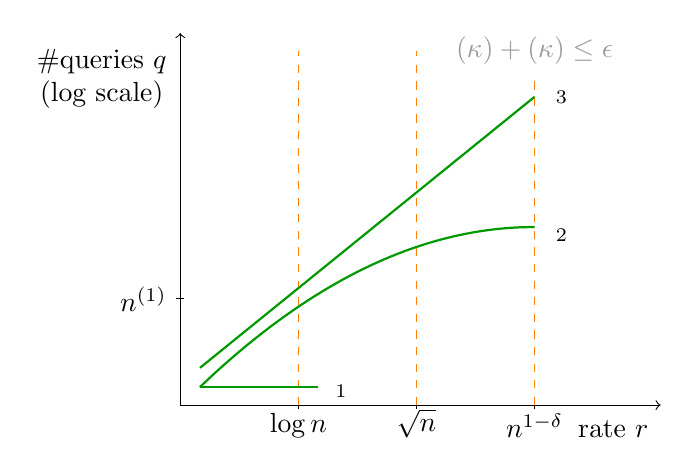
\begin{tikzpicture}[xscale=0.5, yscale=0.45]
  \draw[-{>[scale=2]}] (0,0) to (0,10.5);
  \draw[-{>[scale=2]}] (0,0) to (12.2,0);
  \node[align=center] at (-.1,9.2) [left] {\#queries $q$\\(log scale)};
  \node at (11,-1.2) [above] {rate $r$};

  \draw (3,-.1) to (3,.1);
  \node at (3,-1.2) [above] {$\log n$};
  \draw (6,-.1) to (6,.1);
  \node at (6,-1.2)  [above] {$\sqrt{n}$};
  \draw (9,-.1) to (9,.1);
  \node at (9,-1.2)  [above]  {$n^{1-\delta}$};
  \draw[dashed,color=orange] (9,0) to (9,10);

  \draw[dashed,color=orange] (3,0) to (3,10);

  \draw[dashed,color=orange] (6,0) to (6,10);

  \draw (-.1,3) to (.1,3);
  \node at (-.1,3) [left] {$n^{\landauO(1)}$};

% Nr 1
  \draw[domain=0.5:3.5,smooth,color=green!60!black, thick] plot
  ({\x},{0.5});
%  ({\x},{0.5+0.2*\x-0.3});
  \node at (4.1,0.4) {$\Steg_{1}$};

% Nr 2
  \draw[domain=0.5:9,smooth,color=green!60!black, thick] plot
%  ({\x},{0.8*(\x-0.1*(\x-5)^2)});
  ({\x},{0.2+(-0.0625*(\x^2)+1.125*\x+0.0625 -0.3});
  \node at (9.7,5.1-0.3) {$\Steg_{2}$};

% Nr 3
  \draw[domain=0.5:9,smooth,color=green!60!black, thick] plot
  ({\x},{0.9*(\x+1)-0.3});
  \node at (9.7,9-0.3) {$\Steg_{3}$};

  \node[color=black!40!white,fill=white] at (9,10) {$\InSec(\kappa)+\unrel(\kappa) \le \epsilon$};
\end{tikzpicture}
\caption{Dependencies between rate and number of queries 
of three hypothetical stegosystems of small insecurity and unreliability. 
The systems  $\Steg_2$ and $\Steg_3$ are scalable with respect to
the rate, but $\Steg_1$ is not. 
However to increase the rate in $\Steg_3$ the number of queries increases drastically.
%$\insec$ is defined over all wardens of polynomial time complexity. But there
%it is assumed that the warden has full knowledge about the channel.
}
\label{fig:general:trade:off}
\end{figure}


\section{Security Notions}
In order to define the security of a stegosystem, we first need to
define the abilities that an attacker (the \emph{warden}) has against
the system. We will first define attackers against secret-key
stegosystems that are passive except for the choice of the embedded
message and the corresponding history and then proceed to  present
active attackers against public-key systems that are much more
flexible. The presented security notions will be quite similar to the
cryptographic notions of security against \aclp{CPA+} and security
against \aclp{CCA+}. We will later see in
Chapter~\ref{chap:universal_efficient_secret} that this is no
coincidence. On some channels -- namely those consisting of random
bitstrings -- our definitions coincide. Those are exactly the channels,
where the notions of information encryption and information hiding are
the same.


\subsection*{Chosen-Hiddentext Attackers}
An attacker -- the \myDef{warden} -- $(\Ward_{1},\Ward_{2})$ on the
secret-key stegosystem $\Steg=(\Gen,\SEnc,\SDec)$ is a pair of
\acp{PPTM}. In the \emph{first round}, the algorithm $\Ward_{1}$
produces upon input $1^{\kappa}$ and with oracle access to
$\SEnc^{\chan}_{k}$ and to $\chan$ a message
$m\in \{0,1\}^{\mu(\kappa)}$ and a history $h\in \DomainHistory$. In the
\emph{second round}, $\Ward_{2}$ is either given the stegotexts
containing $m$ or a sequence of completely random documents. Its goal is
to distinguish between those cases. Such an attacker is often called a
\emph{passive} warden, as he only supplies the stegosystem with a
message and a history and then watches the interaction of the
stegoencoder and the stegodecoder. 
This security notion is called
security against \ac{SS-CHA}. Formally, this is defined via the following
experiment $\SSCHA-Dist$.

\myAlgorithm{$\SSCHA-Dist_{(\Ward_{1},\Ward_{2}),\Steg,\chan}(\kappa)$}{Stegosystem 
$\Steg$, Warden $(\Ward_{1},\Ward_{2})$, channel $\chan$, length
$\kappa$}{
\State $k\gets \Gen(1^{\kappa})$
\State $(m,h,s)\gets \Ward_{1}^{\SEnc^{\chan}_{k}, \chan}(1^{\kappa})$
\Comment{$s$ contains \emph{state information}}
\State $b\sgets \{0,1\}$
\If{$b=0$}
\State $d_{1},\ldots,d_{\ell(\kappa)} \gets \SEnc^{\chan}(k,m,h)$
\Else
\For{$i=1,\ldots,\ell(\kappa)$}
\Comment{produce random documents}
\State $d_{i}\gets \chan_{h,n(\kappa)}$; \quad $h := h\mid\mid d_{i}$
\EndFor
\EndIf
\State $b'\gets
\Ward_{2}^{\SEnc^{\chan}_{k},\chan}(1^{\kappa},d_{1},\ldots,d_{\ell(\kappa)},s)$
\If{$b=b'$}
   \AlgReturn{1}
\Else
 \AlgReturn{0}
\EndIf
}{Steganographic-Chosen-Hiddentext-Attack Experiment}

A secret-key stegosystem $\Steg$ is \myDef{\acs{SS-CHA}-secure on $\chan$} if for
every warden $(\Ward_{1},\Ward_{2})$, there is a negligible function
$\negl$ such that
\begin{align*}
  &\Adv_{(\Ward_{1},\Ward_{2}),\Steg,\chan}^{\sscha}(\kappa):=\\
  &\left|\Pr[\SSCHA-Dist_{(\Ward_{1},\Ward_{2}),\Steg,\chan}(\kappa) =
    1] -\frac{1}{2}\right| \leq \negl(\kappa).
\end{align*}

We denote the maximal advantage of a warden $(\Ward_{1},\Ward_{2})$
against the system $\Steg$ on channel $\chan$ as
\begin{align*}
\InSec^{\sscha}_{\Steg,\chan}(\kappa)=\max_{(\Ward_{1},\Ward_{2})}\{\Adv^{\sscha}_{(\Ward_{1},\Ward_{2}),\Steg,\chan}(\kappa)\}
\end{align*}
and call it the \myDef{\acs{SS-CHA}-insecurity} of $\Steg$.

If $\Steg$ is \acs{SS-CHA}-secure on every channel $\chan$, we say that
$\Steg$ is \myDef{universally \acs{SS-CHA}-secure}. 

This steganographic security notion was developed independently by
\citeauthor{katzenbeisser2002defining} in
\cite{katzenbeisser2002defining} and by \citeauthor{hopper2002provably}
in \cite{hopper2002provably}. It was first formalized by
\citeauthor{hopper2002provably} in \cite{hopper2002provably}. 

\subsection*{Chosen-Covertext Attackers}
A \myDef{public-key warden} $(\Ward_{1},\Ward_{2})$ against the public-key
stegosystem $\Steg=(\Gen,\SEnc,\SDec)$ is a pair of \acp{PPTM}. In the
\emph{first round}, the algorithm $\Ward_{1}$ produces upon input $\pk$
and with oracle access to $\chan$ a message $m\in \{0,1\}^{\mu(\kappa)}$
and a history $h\in \DomainHistory$. In the \emph{second round},
$\Ward_{2}$ is either given the stegotexts containing $m$ or a sequence
of completely random documents. To help it distinguish those cases, it
is allowed to \emph{inject arbitrary document} in the channel and
observe the behaviour of the stegodecoder. Clearly, we must prevent it
from decrypting the documents it received. This security notion is known
as security against \acp{SS-CCA}. Formally, this is defined via the
following experiment $\SSCCA-Dist$.


\myAlgorithm{$\SSCCA-Dist_{(\Ward_{1},\Ward_{2}),\Steg,\chan}(\kappa)$}{public-key stegosystem
  $\Steg$, Warden $(\Ward_{1},\Ward_{2})$, channel $\chan$, length $\kappa$}{
\State $(\pk,\sk) \gets \Gen(1^{\kappa})$
\State $(m,h,s) \gets \Ward_{1}^{\SDec_{\sk}, \chan}(\pk)$
\Comment{$s$ contains \emph{state information}}
\State $b \sgets \{0,1\}$
\If{$b=0$}
\State $d_{1},\ldots,d_{\ell(\kappa)} \gets \SEnc^{\chan}(\pk,m,h)$
\Else
\For{$i=1,\ldots,\ell(\kappa)$}
\Comment{produce random documents}
\State $d_{i}\gets \chan_{h,n(\kappa)}$;\quad $h := h\mid\mid d_{i}$
\EndFor
\EndIf
\State $b' \gets
\Ward_{2}^{\SDec_{\sk},\chan}(\pk,d_{1},\ldots,d_{\ell(\kappa)},s)$ 
\If{$\Ward_{2}$ queries $\SDec_{\sk}(d_{1},\ldots,d_{\ell(\kappa)},h)$
  or $b\neq b'$ \label{alg:ss-cca:cond}}
\State  \AlgReturn{0}
\Else
   \AlgReturn{1}
\EndIf
}{Steganographic-Chosen-Covertext-Attack Experiment}

A public-key stegosystem $\Steg$ is \myDef{\acs{SS-CCA}-secure on $\chan$} if for
every public-key warden $(\Ward_{1},\Ward_{2})$, there is a negligible function
$\negl$ such that
\begin{align*}
  &\Adv_{(\Ward_{1},\Ward_{2}),\Steg,\chan}^{\sscca}(\kappa):=\\
  &\left|\Pr[\SSCCA-Dist_{(\Ward_{1},\Ward_{2}),\Steg,\chan}(\kappa) =
    1] -\frac{1}{2}\right| \leq \negl(\kappa).
\end{align*}

We denote the maximal advantage of a warden $(\Ward_{1},\Ward_{2})$
against the system $\Steg$ on channel $\chan$ as
\begin{align*}
\InSec^{\sscca}_{\Steg,\chan}(\kappa)=\max_{(\Ward_{1},\Ward_{2})}\{\Adv^{\sscca}_{(\Ward_{1},\Ward_{2}),\Steg,\chan}(\kappa)\}
\end{align*}
and call it the \myDef{\acs{SS-CCA}-insecurity} of $\Steg$.

If $\Steg$ is \acs{SS-CCA}-secure on every channel $\chan$, we say that
$\Steg$ is \myDef{universally \acs{SS-CCA}-secure}. 

A relaxed notion of \acs{SS-CCA}-security is inspired by the work of
\citeauthor{canetti2003relaxing} \cite{canetti2003relaxing}. This notion
-- called security against \myDef{\acp{SS-RCCA}} -- disallows the warden to mount so
called \emph{replay attacks}. If
$\vec{d}$ is a sequence of documents, a
\myDef{replay} of $\vec{d}$ is a sequence
$\vec{d'}$ with $\vec{d}\neq \vec{d'}$
such that $\SDec_{\sk}(\vec{d},h)=\SDec_{\sk}(\vec{d'},h)$. If
$\Ward_{2}$ is presented with the documents
$\vec{d}=d_{1},\ldots,d_{\ell(\kappa)}$, as in the \acs{SS-CCA}-setting,
the warden is not allowed to decrypt $\vec{d}$, but in addition it is also not
allowed to decrypt any replay of $\vec{d}$. Hence, the experiment
$\SSRCCA-Dist_{(\Ward_{1},\Ward_{2}),\Steg,\chan}(\kappa)$ to describe
\acs{SS-RCCA}-security is the same as for \acs{SS-CCA}-security, but
line \ref{alg:ss-cca:cond} also contains a check, whether any replay of
$d_{1},\ldots,d_{\ell(\kappa)}$ was queried by~$\Ward_{2}$. A
stegosystem is called \myDef{\acs{SS-RCCA}-secure} and
\myDef{universally \acs{SS-RCCA}-secure}, if the corresponding
probabilities concerning $\SSRCCA-Dist$ are negligible. 

Both notions of security against active wardens were first formulated
and formalized by \citeauthor{backes2005active} in
\cite{backes2005active}. 


\section{Relativized Security}
\label{sec:relativized}
One of the most important difference between the formalization of
cryptographic primitives and the formalization of stegosystems is the
presence of the channel. As we will use cryptographic primitives to
construct secure stegosystems, we suddenly bring the notion of the
channel also in the realms of the cryptographic
primitives: In order to base the security of a stegosystem on
the security of a cryptographic primitive, a typical reduction works
along the following lines:
\begin{enumerate}
\item  Suppose that there is a successful warden $\Ward$
on the stegosystem~$\Steg$;
\item  Construct an attacker $\Att$ on the cryptographic
primitive that simulates $\Ward$ on $\Steg$;
\item Prove that the advantage of $\Att$ and $\Ward$
is very similar.
\end{enumerate}
Using such reductions, it is important to note that the attacker $\Att$
on the cryptographic primitives completely simulates the warden $\Ward$
and the encoder of $\Steg$ (assuming a black-box access to the
cryptographic primitive it is based on). As both $\Ward$ and $\Steg$
make calls to the sampling oracle of the channel, $\Att$ also needs
access to those samples.  Hence, the presence of the channel oracle may
influence the security of the used primitives.  This problem was already
observed by \citeauthor{hopper2009provably} in
\cite{hopper2009provably}. There are essentially two solutions to take
the access to the sampling oracle into account:
\begin{itemize}
\item One assumes that the sampling oracle can be simulated in
  \emph{polynomial time}. Hence, the simulation of $\Ward$ and $\Steg$
  can be performed in polynomial time. As the typical requirement is
  that the cryptographic primitives remains secure against attackers
  that run in polynomial time, the security reduction remains valid.

  \citeauthor{backes2005active} choose this solution and write that
  \enquote{In order to avoid technical complications, assume \wlogeneral
    that the sampling oracle is implemented by a probabilistic
    polynomial-time algorithm and therefore does not help and adversary
    beyond its own capabilities \textelp{}} in \cite[page
  213]{backes2005active}. 

\item One assumes that the cryptographic primitive remains secure even
  if the attacker has access to the sampling oracle of the channel
  $\chan$. One then proceeds to define \emph{relativized} versions of
  the common insecurity terms, \eg we could define the advantage
  $\Adv_{\Dist,(\algf,\Gen_{\algf}),\chan}^{\prf}(\kappa)$ of a
  \acl{PRF} $(\algf,\Gen_{\algf})$, where the distinguisher $\Dist$ also
  has access to the sampling oracle of the channel $\chan$ to help it
  distinguish between a totally random function or a pseudorandom one.

  \citeauthor{dedic2009lower} were the first that gave a formal
  definition for this in \cite{dedic2009lower}, but they did not use it
  consistently in their work.  \citeauthor{hopper2009provably}
  implicitly used a similar notion as they assume that
  \enquote{\textelp{} cryptographic primitives remain secure with
    respect to oracles that draw from the marginal channel distribution
    \textelp{}} in \cite[page 665]{hopper2009provably}, but gave no
  formal definition. 


\end{itemize}
%
Note that the assumption that the sampling oracle for channel $\chan$
can be simulated in polynomial time is quite artificial: Arguably, the
single most studied channels for steganography are those containing
multimedia-files such as images or videos\myNote{See \eg the proceedings of
  ACM's IH\&MMSec}. Typically, we do not assume
that one is able to efficiently sample uniformly from the set of all
valid images or videos. This rules out the first possibility. On the
other hand, the second possibility is completely valid, as we have
access to these channels in real-life, but suspect that this access does
not break the security of cryptographic primitives. Due to this
advantage, we will use the second possibility in this work. If $\Pi$ is
a cryptographic primitives (\eg a \acl{PRF}) and $\Att$ an attacker on
this primitive (\eg a distinguisher), we write $\Adv_{\Att,\Pi,\chan}$
to indicate the success probability of $\Att$ against $\Pi$, if $\Att$
also has oracle access to $\chan$, \ie
\begin{align*}
  \Adv_{\Att,\pi,\chan}(\kappa) := \Adv_{\Att^{\chan},\Pi}(\kappa).
\end{align*}
We say that $\Pi$ is \myDef{secure relative to $\chan$}, if for every
attacker $\Att$, there is a negligible function $\negl$ such that
$\Adv_{\Att,\Pi,\chan}(\kappa) \leq \negl(\kappa)$.  Similarly,
$\InSec_{\Pi,\chan}(\kappa)$ is the relativized version of the
insecurity of $\Pi$. 

We also note that \autoref{thm:statistically} also holds in the
relativized setting.


\section{Rejection Sampling}
\label{sec:rejsam}
A very common technique in the design of secure stegosystems called
\myDef{rejection sampling} goes back to an idea of
\citeauthor{anderson1996limits},  presented in
\cite{anderson1996limits}. The basic idea is that Alice samples from the
channel until she finds a document that already encodes the
hiddentext. This was first used by \citeauthor{cachin1998information} in
\cite{cachin1998information} to
construct a secure stegosystem in the information-theoretic sense. We
will also make use of
variants of this approach in
\autoref{chap:universal_nonefficient_secret} and will also show its
limits in \autoref{chap:universal_efficient_secret} and in
\autoref{chap:universal_efficient_public}. Hence, we present this
stegosystem  here in detail. 

In the following, let $F$ be a set of functions that maps input strings
of length $\fin_{F}(\kappa) = n(\kappa)$ (\ie documents) to strings of
length $\fout_{F}(\kappa)$ and $\Pi=(\Gen,\Enc,\Dec)$ be an
\acs{CPA+}-secure \acf{SES}. The stegosystem
$\RejSam^{F,\Pi}=(\Gen^{F,\Pi},\SEnc^{F,\Pi},\SDec^{F,\Pi})$ is defined
as follows:

\myAlgorithm{$\Gen^{F,\Pi}(1^{\kappa})$}{
  length $\kappa$}{
\State $f\sgets F$
\State $k\gets \Gen(1^{\kappa})$
\State \AlgReturn{$(f,k)$}
}{Key-generator of $\RejSam$}

\myAlgorithm{$\SEnc^{F,\Pi}((f,k),m,h)$}{function $f\in F$, key $k$,
  message $m$, history $h$}{
\State $c \gets \Enc(k,m)$
\State parse $c$ into $c_{1}c_{2}\ldots c_{\ell(\kappa)}$ with $|m_{i}|=\fout_{F}(\kappa)$
\For{$j=1,2,\ldots,\ell(\kappa)$}
\State $i := 0$
\Repeat
\State $d \gets \chan_{h,n(\kappa)}$
\State $i := i+1$
\Until{$f(d)=c_{j}$ or $i > \kappa\cdot 2^{\fout_{F}(\kappa)}$}
\State $d_{j} := d$
\State $h := h\mid\mid d_{j}$
\EndFor
\State \AlgReturn{$d_{1},\ldots,d_{\ell(\kappa)}$}
}{Stegoencoder of $\RejSam$}

\myAlgorithm{$\SDec^{F,\Pi}((f,k),h,
  d_{1},\ldots,d_{\ell(\kappa)})$}{function $f\in F$, key $k$,
  documents $d_{1},\ldots,d_{\ell(\kappa)}$, history~$h$}{
\For{$j=1,2,\ldots,\ell(\kappa)$}
\State $c_{j} := f(d_{j})$
\EndFor
\State $c := c_{1}\mid\mid c_{2}\mid\mid \ldots \mid\mid c_{\ell(\kappa)}$
\State $m \gets \Dec(k,c)$
\State \AlgReturn{$m$}
}{Stegodecoder of $\RejSam$}

Clearly, the running time of the encoder is bounded by $\landauO(t_{f}\cdot
\kappa\cdot 2^{\fout_{F}(\kappa)})$, where $t_{f}$ is the time to evaluate the
function $f$. 

In \cite{hopper2009provably}, \citeauthor{hopper2009provably} were the
first to prove the security of this stegosystem in their
complexity-theoretic model, if $F$ is constructed
via a \acf{PRF}.
Their argument was simplified by
\citeauthor{backes2005active} in \cite{backes2005active}, where the
following theorem was proved:
\begin{theorem}[Proposition 1 in \cite{backes2005active}\footnote{The
    exact wording of this proposition and a corresponding proof can be
    found as Proposition 7 in the full version available under the link:
    \url{www.zurich.ibm.com/\textasciitilde cca/papers/pkstego.pdf}}]
\label{thm:backes}
If $\kappa$ is a sufficiently large key-length, then there exists a constant $\eta < 1$
such that
\begin{align*}
D_{S}(P,\chan_{h,n(\kappa)})\leq
  \ell(\kappa)\cdot \left(2^{\fout_{F}(\kappa)-\minent(\chan,n(\kappa))}+\eta^{2^{\fout_{F}(\kappa)}\cdot
  \kappa}\right),
\end{align*}
where $P$ is the distribution generated by the run of the
stegoencoder on a truly random function, \ie 
$\SEnc^{\Fun(\fin_{F}(\kappa),\fout_{F}(\kappa)),\operatorname{id}}(\cdot,m,h)$
upon random choice of $m$ and fixed $h$, where the calls to $\Enc$ and
$\Dec$ are removed (\ie the encoded message $c$ equals $m$).
\end{theorem}

If $F=\{\algf_{k}\mid k\gets \Gen_{\algf}(1^{\kappa})\}$ for a \acl{PRF}
$(\algf,\Gen_{\algf})$ with output length $\fout_{\algf}(\kappa)\leq \log(\kappa)$
and if $\Pi$ is a \ac{CPA+}-secure \acl{SES}, \autoref{thm:backes}
implies that $\RejSam^{F,\Pi}$ is an efficient, universally
reliable and universally secure stegosystem, as no knowledge of $\chan$
is needed by the algorithms.  This is due to the fact that no \ac{PPTM}
can distinguish $F$ from $\Fun(\fin_{F}(\kappa),\fout_{F}(\kappa))$ and no \ac{PPTM}
can distinguish random bitstrings from the ciphertexts of $\Pi$. To
highlight that the set of functions $F$ is coming from a \ac{PRF}
$\algf$, we also denote this stegosystem as $\RejSam^{\algf,\Pi}$.  As
at most $\log(\kappa)$ bits are embedded per document, its rate
$\rate_{\RejSam^{\algf,\pi}}(\kappa)$ is also bounded by $\log(\kappa)$. It
is thus \emph{not} rate-efficient for channels with sufficient
min-entropy. We thus get the following result with $\algf$ and $\Pi$ as
above:

\begin{theorem}[{\cite[Theorems 3 and 4]{hopper2009provably}}]
\label{thm:rejsam:secure}
  There exists a universal stego\-system $\Steg=\RejSam^{\algf,\pi}$ with
  security parameter $\kappa$ that hides a $\ell(\kappa)\cdot \fout_{\algf}(\kappa)$-bit
  message in a sequence of $\ell(\kappa)$
  stego-documents of a channel $\chan$ such that
\begin{align*}
  & \query_{\Steg,\chan}(\kappa) \leq \kappa\cdot 2^{\fout_{\algf}(\kappa)},\\
  & \rate_{\Steg,\chan}(\kappa) = \fout_{\algf}(\kappa),\\
  & \InSec_{\Steg,\chan}(\kappa) \leq \Phi_{\chan}^{\algf,\Pi}(\kappa\cdot
    2^{\fout_{\algf}(\kappa)}), \text{ and}\\
  & \unrel_{\Steg,\chan}(\kappa) \leq \Phi_{\chan}^{\algf,\Pi}(\kappa\cdot 2^{\fout_{\algf}(\kappa)}),
\end{align*}
where
\begin{align*}
  &\Phi_{\chan}^{\algf,\Pi}(t)  :=\\
&\InSec^{\prf}_{(\algf,\Gen_{\algf}),\chan}(t)+\InSec^{\cpad}_{\Pi,\chan}(t)+\negl(\kappa)+2^{\fout_{\algf}(\kappa)-\minent(\chan,n(\kappa))}
\end{align*}
for a negligible function $\negl$. 


%Moreover $\cS$ is stateless 
%stegosystem which does not need any state for synchronization.
\end{theorem}





%%% Local Variables:
%%% TeX-master: "../main"
%%% End:

